\documentclass[11pt,a4paper]{article}
\usepackage[utf8]{inputenc}
\usepackage[vietnamese]{babel}
\usepackage{amsmath,amssymb}
\usepackage[version=4]{mhchem}
\usepackage{geometry}
\geometry{top=1.5cm,bottom=1.2cm,left=1.4cm,right=1.4cm,headheight=28pt,headsep=12pt,footskip=18pt}
\usepackage{graphicx}
\usepackage{xcolor}
\usepackage{tabularx}
\usepackage{array}
\usepackage{tikz}
\usepackage{fancyhdr}
\usepackage{enumitem}
\usepackage{multido}
\usepackage{tcolorbox}
\usepackage{colortbl}

\definecolor{hfRed}{HTML}{D32F2F}
\definecolor{hfGreen}{HTML}{8BC390}
\definecolor{mainGreen}{HTML}{2E7D32}
\definecolor{solBlue}{HTML}{1565C0}
\definecolor{tableGreen}{HTML}{E8F5E9}

\usepackage{ex_test}

\pagestyle{fancy}
\fancyhf{}
\renewcommand{\headrulewidth}{0.75pt}
\renewcommand{\headrule}{\hbox to\headwidth{\color{hfGreen}\leaders\hrule height \headrulewidth\hfill}}
\renewcommand{\footrulewidth}{0.75pt}
\renewcommand{\footrule}{\hbox to\headwidth{\color{hfGreen}\leaders\hrule height \footrulewidth\hfill}}

\fancyhead[L]{\small\itshape\color{hfRed}Tài liệu lưu hành nội bộ}
\fancyhead[R]{\small\color{hfRed}Thầy \textbf{TRẦN VĂN THẠNH} - 0777.470.803}

\fancyfoot[L]{\footnotesize\itshape\color{hfRed}CS1: 6/15 Nguyễn Hoàng, P. Kim Long, TP Huế \quad|\quad CS2: 24 Đặng Thái Thân, TP Huế}
\fancyfoot[R]{\small\textbf{\color{hfRed}Trang \thepage}}

\setlength{\parindent}{0pt}
\setlength{\parskip}{2pt}

\begin{document}

\noindent
\begin{tabularx}{\textwidth}{@{}X r@{}}
\textbf{TRƯỜNG THPT NGUYỄN HUỆ} & \textbf{KIỂM TRA GIỮA KỲ I - NĂM HỌC 2026 - 2027} \\
\textbf{TỔ LÍ - HÓA - CÔNG NGHỆ} & \textbf{Môn: HÓA HỌC, Lớp 12} \\
\textbf{ĐỀ CHÍNH THỨC} & \textbf{Thời gian làm bài: 45 phút} \\
\textit{(Đề có 04 trang)} & \textbf{Mã đề thi: 1202}
\end{tabularx}

\begin{center}
{\color{hfRed}\textbf{\large (BẢN GIÁO VIÊN -- CÓ LỜI GIẢI CHI TIẾT)}}
\end{center}

\vspace{2pt}
\noindent\textbf{Họ và tên thí sinh:} \dotfill \textbf{Số báo danh:} \dots\dots\dots\dots

\vspace{2pt}
\noindent\textit{Lưu ý: Thí sinh không được sử dụng bảng tuần hoàn các nguyên tố hóa học.} \\
\textit{Cho nguyên tử khối của các nguyên tố: H = 1; C = 12; N = 14; O = 16.}
\vspace{2pt}
\hrule height 0.5pt
\vspace{6pt}

\begin{center}
{\color{hfRed}\textbf{\large BẢNG ĐÁP ÁN RÚT GỌN (DÀNH CHO GIÁO VIÊN - MÃ ĐỀ 1202)}}
\end{center}

\noindent{\color{mainGreen}\textbf{1. Phần I: Trắc nghiệm nhiều lựa chọn (12 câu)}}
\begin{center}
\renewcommand{\arraystretch}{1.2}
\begin{tabular}{|c|*{12}{>{\centering\arraybackslash}m{0.9cm}|}}
\hline
\rowcolor{tableGreen}
\textbf{Câu} & \textbf{1} & \textbf{2} & \textbf{3} & \textbf{4} & \textbf{5} & \textbf{6} & \textbf{7} & \textbf{8} & \textbf{9} & \textbf{10} & \textbf{11} & \textbf{12} \\
\hline
\textbf{Đáp án} & \textbf{\color{hfRed}B} & \textbf{\color{hfRed}C} & \textbf{\color{hfRed}B} & \textbf{\color{hfRed}A} & \textbf{\color{hfRed}B} & \textbf{\color{hfRed}C} & \textbf{\color{hfRed}B} & \textbf{\color{hfRed}A} & \textbf{\color{hfRed}A} & \textbf{\color{hfRed}A} & \textbf{\color{hfRed}D} & \textbf{\color{hfRed}B} \\
\hline
\end{tabular}
\end{center}

\vspace{3pt}
\noindent{\color{mainGreen}\textbf{2. Phần II: Trắc nghiệm Đúng / Sai}}
\begin{center}
\renewcommand{\arraystretch}{1.2}
\begin{tabular}{|c|c|c|c|c|c|}
\hline
\rowcolor{tableGreen}
\textbf{Câu} & \textbf{Lệnh hỏi} & \textbf{Ý a)} & \textbf{Ý b)} & \textbf{Ý c)} & \textbf{Ý d)} \\
\hline
\textbf{Câu 1} & Đúng/Sai & \textbf{\color{mainGreen}S} & \textbf{\color{hfRed}Đ} & \textbf{\color{hfRed}Đ} & \textbf{\color{mainGreen}S} \\
\hline
\textbf{Câu 2} & Đúng/Sai & \textbf{\color{mainGreen}S} & \textbf{\color{hfRed}Đ} & \textbf{\color{hfRed}Đ} & \textbf{\color{hfRed}Đ} \\
\hline
\end{tabular}
\end{center}

\vspace{3pt}
\noindent{\color{mainGreen}\textbf{3. Phần III: Trắc nghiệm Trả lời ngắn}}
\begin{center}
\renewcommand{\arraystretch}{1.2}
\begin{tabular}{|c|c|c|c|c|}
\hline
\rowcolor{tableGreen}
\textbf{Câu} & \textbf{Câu 1} & \textbf{Câu 2} & \textbf{Câu 3} & \textbf{Câu 4} \\
\hline
\textbf{Đáp án} & \textbf{\color{hfRed}2} & \textbf{\color{hfRed}3} & \textbf{\color{hfRed}26{,}5} & \textbf{\color{hfRed}145} \\
\hline
\end{tabular}
\end{center}
\vspace{6pt}
\hrule height 0.5pt
\vspace{6pt}

\noindent{\color{mainGreen}\textbf{\Large A. PHẦN TRẮC NGHIỆM (7,0 ĐIỂM)}}
\vspace{4pt}

\noindent{\color{mainGreen}\textbf{\large PHẦN I. Câu hỏi trắc nghiệm nhiều phương án lựa chọn.}} \\
\textit{Thí sinh trả lời từ câu 1 đến câu 12. Mỗi câu hỏi thí sinh chỉ chọn một phương án.}
\vspace{4pt}
\begin{ex}
Chất nào sau đây thuộc loại disaccharide?
\choice
{Amylopectin.}
{\textbf{\color{hfRed}Maltose.}}
{Cellulose.}
{Amylose.}
\loigiai{\textbf{Chọn B.} Carbohydrate được chia làm 3 loại chính: monosaccharide (glucose, fructose), disaccharide (saccharose, maltose) và polysaccharide (tinh bột, cellulose). Vậy maltose thuộc loại disaccharide.}
\end{ex}
\begin{ex}
Số liên kết peptide có trong một phân tử Ala-Gly-Val-Gly-Ala là
\choice
{2.}
{5.}
{\textbf{\color{hfRed}4.}}
{3.}
\loigiai{\textbf{Chọn C.} Phân tử Ala-Gly-Val-Gly-Ala là một pentapeptide được tạo bởi 5 gốc $\alpha$-amino acid, do đó có $5 - 1 = 4$ liên kết peptide.}
\end{ex}
\begin{ex}
Tiến hành thí nghiệm tìm hiểu một số tính chất hóa học của protein theo các bước sau:\\- \textbf{Bước 1:} Cho vào hai ống nghiệm (1) và (2), mỗi ống 2 mL dung dịch lòng trắng trứng.\\- \textbf{Bước 2:} Đun nóng ống nghiệm (1) trên ngọn lửa đèn cồn trong 2 - 3 phút; thêm vài giọt dung dịch \ce{HNO3} đặc vào ống nghiệm (2).\\Phát biểu nào sau đây \textbf{không đúng} ?
\choice
{Sau khi đun nóng, albumin trong ống nghiệm (1) bị đông tụ, tạo thành chất rắn màu trắng.}
{\textbf{\color{hfRed}Hiện tượng ở ống nghiệm (1) chứng tỏ protein đã bị thủy phân hoàn toàn thành các $\alpha$-amino acid.}}
{Sau khi thêm \ce{HNO3} đặc, trong ống nghiệm (2) xuất hiện chất rắn màu vàng.}
{Nếu ngâm ống nghiệm (1) trong nước nóng ở khoảng $80^\circ\text{C}$ trong thời gian thích hợp thì hiện tượng đông tụ protein vẫn xảy ra.}
\loigiai{\textbf{Chọn B.} Đun nóng ống nghiệm (1) gây ra hiện tượng đông tụ protein do biến tính nhiệt, không phải là phản ứng thủy phân protein thành các $\alpha$-amino acid.}
\end{ex}
\begin{ex}
Aniline có thể được điều chế bằng cách khử chất X bằng hỗn hợp Fe và dung dịch \ce{HCl}. Chất X là
\choice
{\textbf{\color{hfRed}\ce{C6H5NO2}.}}
{\ce{C6H5NH2}.}
{\ce{C6H5NO3}.}
{\ce{C6H5N2Cl}.}
\loigiai{\textbf{Chọn A.} Aniline (\ce{C6H5NH2}) được điều chế bằng phản ứng khử nitrobenzene (\ce{C6H5NO2}) bằng hỗn hợp Fe và dung dịch \ce{HCl}.}
\end{ex}
\begin{ex}
Lipid là những hợp chất ...(1)... có trong tế bào sống, không tan trong nước nhưng tan trong dung môi hữu cơ ...(2)...\\Nội dung phù hợp trong các ô trống (1), (2) lần lượt là:
\choice
{vô cơ; phân cực.}
{\textbf{\color{hfRed}hữu cơ; không phân cực.}}
{vô cơ; không phân cực.}
{hữu cơ; phân cực.}
\loigiai{\textbf{Chọn B.} Lipid là những hợp chất hữu cơ có trong tế bào sống, không tan trong nước nhưng tan trong các dung môi hữu cơ không phân cực (hoặc kém phân cực).}
\end{ex}
\begin{ex}
Loại protein nào sau đây tan được trong nước?
\choice
{Keratin (có ở tóc, móng).}
{Collagen (có ở da, sụn).}
{\textbf{\color{hfRed}Hemoglobin (có ở máu).}}
{Myosin (có ở cơ bắp).}
\loigiai{\textbf{Chọn C.} Hemoglobin trong máu là protein dạng hình cầu, tan được trong nước tạo dung dịch keo. Keratin, collagen, myosin là các protein hình sợi, không tan trong nước.}
\end{ex}
\begin{ex}
Số nhóm amino (\ce{-NH2}) có trong một phân tử Lysine là
\choice
{3.}
{\textbf{\color{hfRed}2.}}
{1.}
{4.}
\loigiai{\textbf{Chọn B.} Lysine có công thức cấu tạo: \ce{H2N-[CH2]4-CH(NH2)-COOH}, chứa 2 nhóm amino (\ce{-NH2}) và 1 nhóm carboxyl (\ce{-COOH}).}
\end{ex}
\begin{ex}
Cho các chất hữu cơ sau: ethyl acetate (\ce{CH3COOC2H5}), methyl formate (\ce{HCOOCH3}), propanoic acid (\ce{C2H5COOH}) và propan-1-ol (\ce{CH3CH2CH2OH}). Biết nhiệt độ sôi của các chất trên ở $1\text{ atm}$ (không theo thứ tự) là: $97{,}2^\circ\text{C}$; $77{,}1^\circ\text{C}$; $32{,}0^\circ\text{C}$ và $141^\circ\text{C}$. Nhiệt độ sôi của ethyl acetate là bao nhiêu?
\choice
{\textbf{\color{hfRed}$77{,}1^\circ\text{C}$.}}
{$32{,}0^\circ\text{C}$.}
{$141^\circ\text{C}$.}
{$97{,}2^\circ\text{C}$.}
\loigiai{\textbf{Chọn A.} Nhiệt độ sôi: Acid carboxylic cao nhất ($141^\circ\text{C}$), sau đó đến alcohol ($97{,}2^\circ\text{C}$). Hai ester không tạo liên kết hydro, ethyl acetate ($M = 88$) có phân tử khối lớn hơn methyl formate ($M = 60$) nên nhiệt độ sôi của ethyl acetate là $77{,}1^\circ\text{C}$ (methyl formate là $32{,}0^\circ\text{C}$).}
\end{ex}
\begin{ex}
Saccharose có nhiều trong nguyên liệu thực phẩm nào sau đây?
\choice
{\textbf{\color{hfRed}Thân cây mía.}}
{Gạo.}
{Mật ong.}
{Lúa mạch.}
\loigiai{\textbf{Chọn A.} Saccharose có nhiều nhất trong thân cây mía (đường mía, chiếm 13 - 15\%), củ cải đường và hoa thốt nốt.}
\end{ex}
\begin{ex}
Tiến hành thí nghiệm theo các bước sau:\\- \textbf{Bước 1:} Cho vào cốc thuỷ tinh chịu nhiệt khoảng 5 gam dầu dừa và 10 mL dung dịch \ce{NaOH} 40\%.\\- \textbf{Bước 2:} Đun hỗn hợp trong khoảng 10 phút, liên tục khuấy bằng đũa thuỷ tinh và thỉnh thoảng thêm nước.\\- \textbf{Bước 3:} Rót hỗn hợp vào cốc thuỷ tinh chứa khoảng 70 mL dung dịch \ce{NaCl} bão hoà, khuấy nhẹ rồi để yên.\\Phát biểu nào sau đây về thí nghiệm trên \textbf{không đúng} ?
\choice
{\textbf{\color{hfRed}Ở bước 1, nếu thay dầu dừa bằng mỡ lợn thì sản phẩm thu được sau bước 3 hoàn toàn giống nhau.}}
{Sau bước 3, xuất hiện lớp chất rắn màu trắng, chủ yếu là xà phòng, nổi lên trên bề mặt.}
{Trong thí nghiệm trên, có xảy ra phản ứng xà phòng hóa chất béo.}
{Ở bước 3, thêm dung dịch \ce{NaCl} bão hòa là để tách muối của acid béo ra khỏi hỗn hợp.}
\loigiai{\textbf{Chọn A.} Dầu dừa chứa chủ yếu gốc acid lauric, trong khi mỡ lợn chứa các gốc acid palmitic, stearic, oleic... Do đó muối sodium của acid béo (xà phòng) thu được có thành phần khác nhau, không thể hoàn toàn giống nhau.}
\end{ex}
\begin{ex}
Protein là hợp chất cao phân tử được cấu tạo từ một hay nhiều chuỗi
\choice
{polysaccharide.}
{lipid.}
{nucleic acid.}
{\textbf{\color{hfRed}polypeptide.}}
\loigiai{\textbf{Chọn D.} Protein là hợp chất cao phân tử được cấu tạo từ một hay nhiều chuỗi polypeptide.}
\end{ex}
\begin{ex}
Monosaccharide X có trong nhiều loại trái cây (táo, lựu, nho, lê,...), trong một số loại rau củ (cà rốt, củ cải đường,...) và có nhiều nhất trong mật ong. Tên gọi của X là
\choice
{maltose.}
{\textbf{\color{hfRed}fructose.}}
{saccharose.}
{glucose.}
\loigiai{\textbf{Chọn B.} Fructose là monosaccharide có vị ngọt sắc, có nhiều trong trái cây và chiếm khoảng 40\% khối lượng trong mật ong.}
\end{ex}

\vspace{6pt}
\noindent{\color{mainGreen}\textbf{\large PHẦN II. Câu trắc nghiệm đúng sai.}} \\
\textit{Thí sinh trả lời từ câu 1 đến câu 2. Trong mỗi ý a), b), c), d) ở mỗi câu, thí sinh chọn đúng hoặc sai.}
\vspace{4pt}

\begin{ex}
Chất X có hai thành phần chính, cấu tạo một đoạn mạch của mỗi thành phần được biểu diễn như hình sau:
\begin{center}
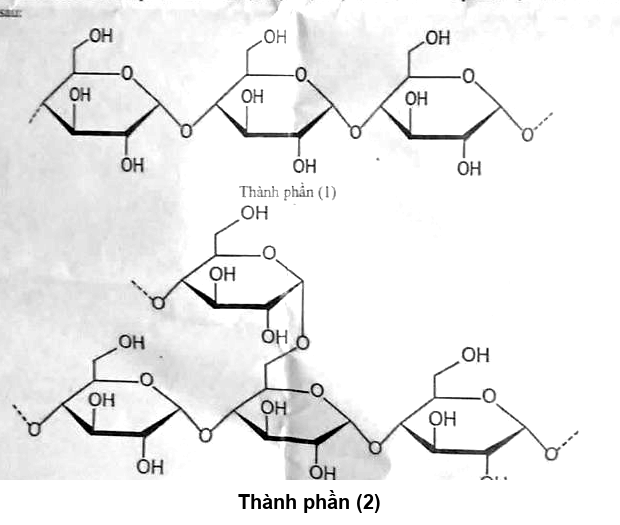
\includegraphics[width=0.72\textwidth]{images_gk1_hoa12_nguyenhue_1202/cau1_p2_tinh_bot.png}
\end{center}
\choiceTF
Thành phần (2) có cấu trúc phân nhánh do sự xuất hiện của các liên kết $\beta$-1,6-glycoside.
\True X là một polysaccharide.
\True Trong thực vật, X có chủ yếu trong củ, quả hay hạt.
Tiến hành lần lượt các thí nghiệm của X (ở dạng dung dịch keo nhớt) với: dung dịch \ce{AgNO3}/\ce{NH3}, đun nóng (1); dung dịch \ce{I2} (2); \ce{Cu(OH)2} (3); dung dịch \ce{HCl}, đun nóng (4); dung dịch \ce{NaOH} (5). Số thí nghiệm X có phản ứng là 3.
\loigiai{
Chất X là tinh bột, gồm amylose (thành phần 1, không phân nhánh) và amylopectin (thành phần 2, phân nhánh).\\
\textbf{Ý a) SAI.} Điểm phân nhánh của amylopectin là liên kết $\alpha$-1,6-glycosidic, không phải $\beta$-1,6-glycoside.\\
\textbf{Ý b) ĐÚNG.} Tinh bột là polymer thiên nhiên thuộc loại polysaccharide có CTPT \ce{(C6H10O5)_n}.\\
\textbf{Ý c) ĐÚNG.} Tinh bột là chất dinh dưỡng dự trữ của thực vật, tích tụ nhiều trong hạt, củ, quả.\\
\textbf{Ý d) SAI.} Trong 5 thí nghiệm, chỉ có (2) (tạo hợp chất màu xanh tím với \ce{I2}) và (4) (thủy phân trong môi trường acid khi đun nóng) xảy ra phản ứng/biến đổi đặc trưng. Tinh bột không tráng bạc (1), không hòa tan \ce{Cu(OH)2} ở nhiệt độ thường (3), không bị thủy phân trong kiềm (5). Vậy số thí nghiệm có phản ứng là 2, không phải 3.
}
\end{ex}

\begin{ex}
Cho các phát biểu sau về ba chất: aniline, glycine và valine.
\choiceTF
Tương tự glycine, ở $\text{pH} = 11$, valine di chuyển về cực âm (-) khi đặt trong điện trường.
\True Có 2 chất là amino acid thiên nhiên.
\True Ở điều kiện thường, aniline là chất lỏng, ít tan trong nước.
\True Cả glycine và valine đều tác dụng được với dung dịch \ce{HCl} và dung dịch \ce{NaOH}.
\loigiai{
\textbf{Ý a) SAI.} Tại $\text{pH} = 11$ ($\text{pH} > \text{pI} \approx 6$), glycine và valine tồn tại ở dạng anion carboxylate \ce{H2N-CH(R)-COO^-}, mang điện tích âm nên di chuyển về \textbf{cực dương (+)}, không phải cực âm.\\
\textbf{Ý b) ĐÚNG.} Glycine và valine là hai $\alpha$-amino acid thiên nhiên. Aniline là amine thơm.\\
\textbf{Ý c) ĐÚNG.} Aniline là chất lỏng không màu (để lâu bị nâu đen), rất ít tan trong nước.\\
\textbf{Ý d) ĐÚNG.} Cả glycine và valine đều là các amino acid có tính chất lưỡng tính nên phản ứng với cả acid mạnh (\ce{HCl}) và base mạnh (\ce{NaOH}).
}
\end{ex}

\vspace{6pt}
\noindent{\color{mainGreen}\textbf{\large PHẦN III: Câu trắc nghiệm yêu cầu trả lời ngắn.}} \\
\textit{Thí sinh trả lời từ câu 1 đến câu 4.}
\vspace{4pt}

\begin{ex}
Trong số các chất sau: oleic acid, sodium alkylsulfate, triolein, ethyl acetate, sodium stearate, glucose, có bao nhiêu chất có tính chất giặt rửa?
\shortans{2}
\loigiai{
\textbf{Trả lời: 2}\\
Gồm 2 chất: sodium alkylsulfate (chất giặt rửa tổng hợp) và sodium stearate (xà phòng).
}
\end{ex}

\begin{ex}
Cho các chất sau: \ce{CH3-NH2}, \ce{H2N-CH2-COOH}, \ce{CH3-CH2-NO2}, \ce{CH3-NH-CH3}, \ce{C6H5-CH2-NH2}, \ce{CH3-NH3Cl}. Số chất thuộc loại amine là bao nhiêu?
\shortans{3}
\loigiai{
\textbf{Trả lời: 3}\\
Gồm 3 chất: \ce{CH3-NH2} (methylamine), \ce{CH3-NH-CH3} (dimethylamine), \ce{C6H5-CH2-NH2} (benzylamine).
}
\end{ex}

\begin{ex}
Thủy phân hoàn toàn tetrapeptide mạch hở X thu được hỗn hợp gồm: glycine, alanine và valine với tỉ lệ mol tương ứng là 2:1:1. Phần trăm khối lượng của oxygen có trong X là bao nhiêu (làm tròn kết quả đến hàng phần mười)?
\shortans{26{,}5}
\loigiai{
\textbf{Trả lời: 26{,}5}\\
- Tetrapeptide X tạo từ 2 gốc Gly, 1 gốc Ala và 1 gốc Val:\\
CTPT của X: \ce{C12H22N4O5} ($M = 12 \times 12 + 22 + 14 \times 4 + 16 \times 5 = 302\text{ g/mol}$).\\
- Phần trăm khối lượng oxygen trong X:
$\%m_{\text{O}} = \frac{5 \times 16}{302} \times 100\% = 26{,}490\% \approx \mathbf{26{,}5\%}$.
}
\end{ex}

\begin{ex}
Học sinh tiến hành các thí nghiệm về tính chất hóa học của amine và nêu hiện tượng xảy ra tương ứng như sau:\\
- \textbf{Thí nghiệm 1:} Cho từ từ nước bromine vào ống nghiệm đựng dung dịch aniline và lắc đều thấy xuất hiện chất rắn màu trắng.\\
- \textbf{Thí nghiệm 2:} Cho dung dịch methylamine vào ống nghiệm đựng dung dịch iron (III) chloride thấy xuất hiện chất rắn màu trắng hơi xanh sau đó hóa nâu đỏ.\\
- \textbf{Thí nghiệm 3:} Nhỏ một giọt dung dịch aniline lên mẩu giấy quỳ tím đặt trên mặt kính đồng hồ thấy giấy quỳ chuyển sang màu xanh.\\
- \textbf{Thí nghiệm 4:} Nhỏ từ từ dung dịch methylamine vào ống nghiệm đựng kết tủa copper (II) hydroxide thấy kết tủa tan ra tạo dung dịch phức chất có màu xanh lam.\\
- \textbf{Thí nghiệm 5:} Cho từ từ dung dịch ethylamine vào ống nghiệm đựng dung dịch nitrous acid thấy có bọt khí không màu thoát ra.\\
Liệt kê các thí nghiệm có hiện tượng phù hợp tương ứng theo thứ tự tăng dần của số thứ tự (ví dụ: 134, 23, ...).
\shortans{145}
\loigiai{
\textbf{Trả lời: 145}\\
- Thí nghiệm 1: Phù hợp (kết tủa trắng 2,4,6-tribromoaniline).\\
- Thí nghiệm 2: Không phù hợp (tạo ngay kết tủa nâu đỏ \ce{Fe(OH)3}, không qua giai đoạn trắng hơi xanh).\\
- Thí nghiệm 3: Không phù hợp (aniline không làm đổi màu quỳ tím).\\
- Thí nghiệm 4: Phù hợp (hòa tan \ce{Cu(OH)2} tạo phức \ce{[Cu(CH3NH2)4](OH)2} màu xanh lam).\\
- Thí nghiệm 5: Phù hợp (\ce{C2H5NH2 + HNO2 -> C2H5OH + N2 ^ + H2O}, thoát khí \ce{N2} không màu).\\
$\Rightarrow$ Các thí nghiệm phù hợp: 1, 4, 5. Ghi: \textbf{145}.
}
\end{ex}

\vspace{6pt}
\noindent{\color{mainGreen}\textbf{\Large B. PHẦN TỰ LUẬN (3,0 ĐIỂM)}}
\vspace{4pt}

\noindent\textbf{Câu 1. (1,0 điểm)} Ester X có công thức phân tử là \ce{C4H8O2}. Xà phòng hóa hoàn toàn X thu được muối Y và alcohol Z. Biết số nguyên tử carbon trong một phân tử Z lớn hơn số nguyên tử carbon trong một phân tử Y. Viết tất cả các công thức cấu tạo thu gọn có thể có của X và tên gọi tương ứng (mỗi công thức cấu tạo chỉ ghi một tên gọi).

\begin{tcolorbox}[colback=white,colframe=solBlue,arc=1mm,boxrule=0.5pt,top=2mm,bottom=2mm,left=3mm,right=3mm]
{\color{solBlue}\textbf{► Lời giải chi tiết:}}\\
- Ester X đơn chức, mạch hở no có CTPT \ce{C4H8O2}, công thức dạng \ce{RCOOR'}.\\
Phương trình phản ứng xà phòng hóa: \ce{RCOOR' + NaOH -> RCOONa (Y) + R'OH (Z)}.\\
- Gọi số nguyên tử C trong Y là $C_Y$ và trong Z là $C_Z$. Ta có: $C_Y + C_Z = 4$.\\
- Theo giả thiết $C_Z > C_Y \Rightarrow C_Z > 2 \Rightarrow C_Z = 3$ và $C_Y = 1$.\\
- Muối Y có 1 carbon là \ce{HCOONa} (sodium formate).\\
- Alcohol Z có 3 carbon là \ce{C3H7OH}, tương ứng có 2 đồng phân cấu tạo của gốc R':
\begin{itemize}[noitemsep,topsep=1pt]
\item \ce{HCOOCH2CH2CH3}: propyl formate
\item \ce{HCOOCH(CH3)2}: isopropyl formate
\end{itemize}
\end{tcolorbox}

\vspace{6pt}
\noindent\textbf{Câu 2. (1,0 điểm)} Cellulose nitrate (nitrocellulose) có nhiều ứng dụng trong đời sống. Khi cho cellulose tác dụng với hỗn hợp \ce{HNO3} đặc và \ce{H2SO4} đặc trong điều kiện thích hợp, tùy theo mức độ phản ứng, số lượng nhóm nitrate (\ce{-ONO2}) được tạo thành ở các mắt xích có thể khác nhau.\\
a) Giải thích vì sao mỗi mắt xích \ce{C6H10O5} của cellulose có thể phản ứng với tối đa 3 phân tử \ce{HNO3}.\\
b) Viết phương trình hóa học của phản ứng tạo thành cellulose trinitrate, một chất được sử dụng trong sản xuất thuốc súng không khói.

\begin{tcolorbox}[colback=white,colframe=solBlue,arc=1mm,boxrule=0.5pt,top=2mm,bottom=2mm,left=3mm,right=3mm]
{\color{solBlue}\textbf{► Lời giải chi tiết:}}\\
a) \textbf{Giải thích:}\\
Mỗi mắt xích \ce{C6H10O5} trong phân tử cellulose có 3 nhóm hydroxyl (\ce{-OH}) tự do, được viết ở dạng công thức: \ce{[C6H7O2(OH)3]_n}. Trong phản ứng ester hóa với \ce{HNO3} đặc (xúc tác \ce{H2SO4} đặc, $t^\circ$), mỗi nhóm \ce{-OH} có thể bị ester hóa bởi một phân tử \ce{HNO3} để tạo thành nhóm ester nitrate (\ce{-ONO2}). Do chỉ có tối đa 3 nhóm \ce{-OH} tự do ở mỗi mắt xích nên mỗi mắt xích phản ứng tối đa với 3 phân tử \ce{HNO3}.\\
b) \textbf{Phương trình hóa học điều chế cellulose trinitrate:}\\
\centerline{\ce{[C6H7O2(OH)3]_n + 3n HNO3 ->[H2SO4 \text{ đặc}, t^o] [C6H7O2(ONO2)3]_n + 3n H2O}}
\end{tcolorbox}

\vspace{6pt}
\noindent\textbf{Câu 3. (1,0 điểm)} Một học sinh tiến hành thí nghiệm thử tính chất của carbohydrate như sau:\\
\textbf{Bước 1:} Cho khoảng 5 mL dung dịch hồ tinh bột 1\% vào ống nghiệm (1). Sau đó thêm khoảng 1 mL dung dịch \ce{HCl} 1 M vào, lắc đều.\\
\textbf{Bước 2:} Đặt ống nghiệm (1) trong một cốc thuỷ tinh chứa nước nóng, đun cách thuỷ trong 10 phút. Sau đó để nguội.\\
\textbf{Bước 3:} Thêm từ từ \ce{NaHCO3} vào ống nghiệm (1) đến khi ngừng sủi bọt khí.\\
\textbf{Bước 4:} Chia dung dịch thu được ở ống nghiệm (1) thành hai phần gần bằng nhau, cho vào ống nghiệm (2) và (3).\\
\textbf{Bước 5:} Cho 0,5 mL dung dịch \ce{CuSO4} 5\% vào ống nghiệm chứa 2 mL dung dịch \ce{NaOH} 10\%, lắc nhẹ.\\
\textbf{Bước 6:} Đổ dung dịch trong ống nghiệm (2) vào ống nghiệm chứa \ce{Cu(OH)2} (thu được ở bước 5) và lắc đều.\\
\textbf{Bước 7:} Đổ dung dịch trong ống nghiệm (3) vào ống nghiệm chứa nước bromine loãng.\\
Viết phương trình hóa học của các phản ứng xảy ra ở các bước 2, 3, 6 và 7 trong thí nghiệm trên (ghi rõ điều kiện phản ứng nếu có).

\begin{tcolorbox}[colback=white,colframe=solBlue,arc=1mm,boxrule=0.5pt,top=2mm,bottom=2mm,left=3mm,right=3mm]
{\color{solBlue}\textbf{► Lời giải chi tiết:}}\\
- \textbf{Bước 2 (Thủy phân tinh bột):}\\
\centerline{\ce{(C6H10O5)_n + n H2O ->[H^+, t^o] n C6H12O6}\text{ (glucose)}}\\
- \textbf{Bước 3 (Trung hòa lượng \ce{HCl} dư bằng \ce{NaHCO3}):}\\
\centerline{\ce{HCl + NaHCO3 -> NaCl + CO2 ^ + H2O}}\\
- \textbf{Bước 6 (Phản ứng hòa tan \ce{Cu(OH)2} tạo phức màu xanh lam):}\\
\centerline{\ce{2 C6H12O6 + Cu(OH)2 -> (C6H11O6)2Cu + 2 H2O}}\\
- \textbf{Bước 7 (Phản ứng oxi hóa glucose bằng nước bromine):}\\
\centerline{\ce{CH2OH[CHOH]4CHO + Br2 + H2O -> CH2OH[CHOH]4COOH + 2 HBr}}\\
\textit{(hoặc viết: \ce{C6H12O6 + Br2 + H2O -> C6H12O7 + 2 HBr})}
\end{tcolorbox}

\vspace{8pt}
\begin{center}
\textbf{--- HẾT ---} \\
\textit{\small Thí sinh không được sử dụng tài liệu; giám thị không giải thích gì thêm.}
\end{center}
\end{document}
